\newcommand{\blat}{2 cm}
\newcommand{\sqth}{1.73205080757}
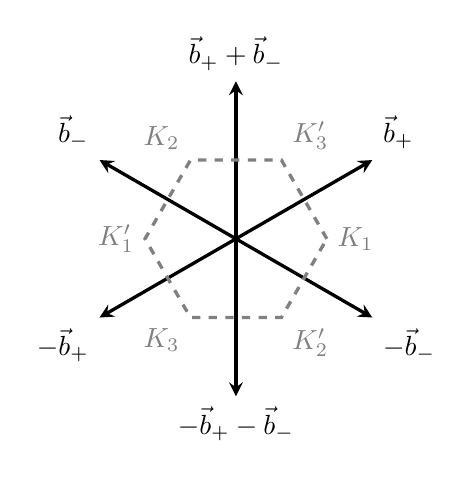
\begin{tikzpicture}[>=stealth,
	RLV/.style={very thick,->,color=black},
	BZ/.style ={very thick, color=gray, dashed}]

	% The reciprocal lattice vectors that go to the 6 nearest neighbors
	\draw[RLV] (0,0) -- ( 30:\blat) node[anchor=south west]{$\vec{b}_+$};
	\draw[RLV] (0,0) -- ( 90:\blat) node[anchor=south     ]{$\vec{b}_+ + \vec{b}_-$};
	\draw[RLV] (0,0) -- (150:\blat) node[anchor=south east]{$\vec{b}_-$};
	\draw[RLV] (0,0) -- (210:\blat) node[anchor=north east]{$-\vec{b}_+$};
	\draw[RLV] (0,0) -- (270:\blat) node[anchor=north     ]{$-\vec{b}_+ - \vec{b}_-$};
	\draw[RLV] (0,0) -- (330:\blat) node[anchor=north west]{$-\vec{b}_-$};

	%The constructed first Brillouin zone
	\draw[BZ]
		(  0:\blat/\sqth) node[anchor=west      ]{$\bm{K_1} $} --
		( 60:\blat/\sqth) node[anchor=south west]{$\bm{K_3'}$} --
		(120:\blat/\sqth) node[anchor=south east]{$\bm{K_2}$} -- 
		(180:\blat/\sqth) node[anchor=east      ]{$\bm{K_1'}$} -- 
		(240:\blat/\sqth) node[anchor=north east]{$\bm{K_3}$} -- 
		(300:\blat/\sqth) node[anchor=north west]{$\bm{K_2'}$} -- 
		(  0:\blat/\sqth);

\end{tikzpicture}